\documentclass{article}
\usepackage[T1]{fontenc}
\usepackage{lmodern}
\usepackage{graphicx}
\usepackage{amsmath,amssymb}
\usepackage[a4paper,margin=2cm]{geometry}
\usepackage[absolute,overlay]{textpos}
\setlength{\TPHorizModule}{1mm}
\setlength{\TPVertModule}{1mm}
\usepackage[indonesian]{babel}
\usepackage{hyperref}
\setlength{\emergencystretch}{2em}
% unit: Halaman 2

\begin{document}

% === Halaman 2 (llm) ===

\section*{Pendahuluan}

\vspace{129.79mm}

\begin{itemize}
    \item Algoritma Elgamal dibuat oleh Taher Elgamal (1985). Pertama kali dikemukakannya di dalam makalah berjudul "A public key cryptosystem and a signature scheme based on discrete logarithms", dimuat di dalam \href{https://ieeexplore.ieee.org/document/1056437}{IEEE Transactions on Information Theory} ( Volume: 31, \href{https://ieeexplore.ieee.org/document/1056437}{Issue: 4}, July 1985)
\end{itemize}

\vspace{10mm}

% deskripsi: Foto profil Taher Elgamal dengan teks 'Taher Elgamal Founder, Securify'
% bbox normalisasi: [0.1130, 0.4880, 0.4920, 0.9060]
\begin{textblock*}{79.59mm}(23.73mm,144.94mm)
\noindent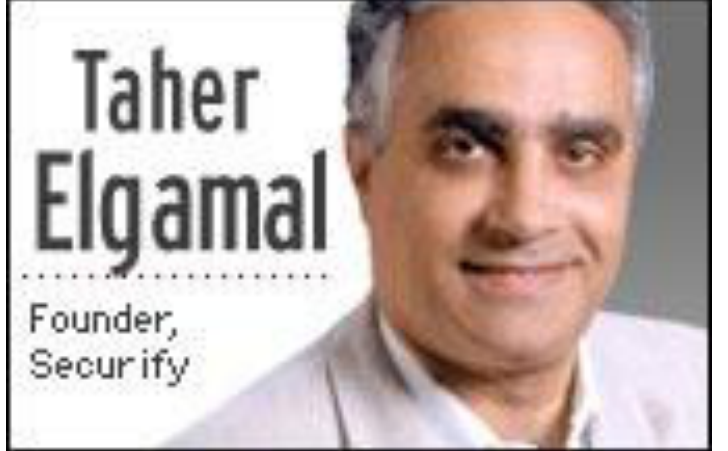
\includegraphics[width=79.59mm,height=124.15mm]{../../images/llm/page_002_img_01.png}%
\end{textblock*}

% deskripsi: Foto Taher Elgamal saat menerima Lifetime Achievement Award di RSACONFERENCE 2009
% bbox normalisasi: [0.5210, 0.4880, 0.9010, 0.9250]
\begin{textblock*}{79.80mm}(109.41mm,144.94mm)
\noindent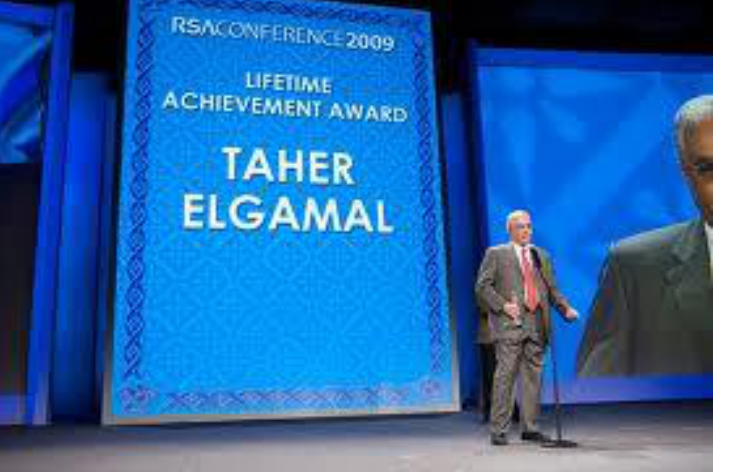
\includegraphics[width=79.80mm,height=129.79mm]{../../images/llm/page_002_img_02.png}%
\end{textblock*}

\end{document}
